\documentclass[onecolumn, draftclsnofoot,10pt, compsoc]{article}
\usepackage{graphicx}
\usepackage{url}
\usepackage{lscape}
\usepackage{setspace}
\usepackage{parskip}
\usepackage{geometry}
\usepackage{listings}
\usepackage{subfiles}
\usepackage{pdfpages}
\geometry{textheight=9.5in, textwidth=7in}

% 1. Fill in these details
\def \CapstoneTeamName{AgBizClimate}
\def \CapstoneTeamNumber{26}
\def \GroupMemberOne{}%Your Name Here
\def \CapstoneProjectName{ Linking Seasonal Weather Data to AgBizClimate\texttrademark}
\def \CapstoneSponsorCompany{ Oregon State University}
\def \CapstoneSponsorPerson{ Clark Seavert}

% 2. Uncomment the appropriate line below so that the document type works
\def \DocType{		%Software Requirements Document
				%Requirements Document
				%Technology Review
				%Design Document
				Final Document
				}

\newcommand{\NameSigPair}[1]{\par
\makebox[2.75in][r]{#1} \hfil 	\makebox[3.25in]{\makebox[2.25in]{\hrulefill} \hfill		\makebox[.75in]{\hrulefill}}
\par\vspace{-12pt} \textit{\tiny\noindent
\makebox[2.75in]{} \hfil		\makebox[3.25in]{\makebox[2.25in][r]{Signature} \hfill	\makebox[.75in][r]{Date}}}}
% 3. If the document is not to be signed, uncomment the RENEWcommand below
%\renewcommand{\NameSigPair}[1]{#1}

%%%%%%%%%%%%%%%%%%%%%%%%%%%%%%%%%%%%%%%
\begin{document}
\begin{titlepage}
    \pagenumbering{gobble}
    \begin{singlespace}
        \hfill
        % 4. If you have a logo, use this includegraphics command to put it on the coversheet.
        %\includegraphics[height=4cm]{CompanyLogo}
        \par\vspace{.2in}
        \centering
        \scshape{
            \huge CS Capstone \DocType \par
            {\large\today}\par
            \vspace{.5in}
            \textbf{\Huge\CapstoneProjectName}\par
            \vfill
            {\large Prepared for}\par
            \Huge \CapstoneSponsorCompany\par
            \vspace{5pt}
            {\Large\NameSigPair{\CapstoneSponsorPerson}\par}
            {\large Prepared by }\par
            Group\CapstoneTeamNumber\par
            % 5. comment out the line below this one if you do not wish to name your team
            %\CapstoneTeamName\par
            \vspace{5pt}
            {\Large
                \NameSigPair{\GroupMemberOne}\par
            }
            \vspace{20pt}
        }
        \begin{abstract}
			The purpose of this document is to provide documentation regarding the \textit{AgBizClimate} project. We will start off the document by giving a general overview of the \textit{AgBizClimate Project}. This will inclue information about the goals of the project, and information about the project stakeholders. Next we have our requirements document. In this section we will also discuss how our requirements have changed over the last several terms. Next we will be discussing the design document. In this section we will first display our original design document. We will then discuss how our design has changed over the term. After the design document we will display the tech review. Next, we will also display the project poster. Finally we will provide some project documentation regarding how project setup, running the project, how the project works and guids for any API's we are using. After this we will discuss any technical resources for learning more about the technologies that our project uses. Finally, We will end this document with our conclusions and reflections section. This section will involve reflecting on this project and discussing what went well and what didn't go well.\\
        \end{abstract}
    \end{singlespace}
\end{titlepage}
\newpage
\pagenumbering{arabic}
\tableofcontents
% 7. uncomment this (if applicable). Consider adding a page break.
%\listoffigures 
\newpage
%\listoftables
\clearpage

% 8. now you write!
% Will need to review this section to make sure its accurate and that it covers all the bullet points in the 
% requirements for this section.
\section{Introduction}
		\subsection{Purpose}
		This SRS describes the requirements and specifications of the AgBizClimate\texttrademark web application. This document will explain the functional features of this web application. This includes the interface details, design constraints and considerations such as performance characteristics. This SRS is intended to outline how we will proceed with the development of the \textit{AgBizClimate} system.\\

		\subsection{Scope}
			This project is a part of a much larger AgBiz Logic\texttrademark program. However, the purpose of this project is to add a short term climate tool to the \textit{AgBizClimate} module. This limits the scope of the project to the \textit{AgBizClimate} Module. Additionally, we will only be adding the short term climate data tool as the long term climate data tool already exists.\\

		\subsection{Definitions, Acronyms and Abbreviations}
			REST - Representation State Transfer, This is a type of architecture that manages preforms operations on the state of the program. This is especially popular in web development.\\
			API- Application Programming Interface. This is a piece of software that allows a connection to another piece of software providing some sort of service.\\
			Thredds Data Server - This is a web server that provides meta-data and data access for scientific data sets using OPeNDAP along with some other remote data access protocols.\\
			OPeNDAP - Open-source Project for a Network Data Access Protocol. This is the protocol we will be using to retrieve the data sets from the Thredds data server.\\
			NMME - North American Multi-Model Ensemble. This is a data set that brings together a variety of different weather models into one data set.\\
			Climate Scenario - This is a theoretical calculation of yields, inputs and of the overall budget for one situation based on the climate data.\\
			NETCDF - This is a file storage format for large scientific data sets especially good for any data that is referenced on a grid and related to is geo-location.\\
			SQL Database - This is a relational database that makes storing and accessing data easy.\\
			Container - A virtualized operating system that is used to host and deploy web development projects. This allows projects to be easily portable between different operating systems and platforms.\\
			Mount Bind - This is the practice of mounting a directory from the native os to the container such that if either the container or the native operating system. This allows changes in the files to be reflected in both the container and the native operating system.\\
			

			\renewcommand\refname{\vskip -1cm}
		\subsection{References}

		\nocite{*}
    \bibliographystyle{IEEEtran}
    \bibliography{IEEEabrv,References}


		\subsection{Overview}
			Seasonal climate is one of the essential factors that affects agricultural production. As a module of \textit{AgBiz Logic}, \textit{AgBizClimate} delivers essential information about climate change to farmers, and help professionals to develop management pathways that best fit their operations under a changing climate. This project aims to link the seasonal climate data from the NMME data set to \textit{AgBiz Logic} so that it can provide changes in net returns of crop and livestock enterprises through powerful graphics and tables. \\
			Currently \textit{AgBizClimate} has a long-term climate tool but no such tool exists for short term climate data. We will implement a tool to extract short-term climate data from the NMME data set, display it to the user and allow the user to adjust crop and livestock yields or quality of products sold and, production inputs. Moreover, a landing tool will be developed to allow users to switch between short-term seasonal tool and long-term climate data tool.\\
			
	\subsection {Product Functions}
				\textit{AgBizClimate} is a web based decision tool that will allow users to gain specific insight on how localized climate data for the next seven months will affect their crop and livestock yields or quality of products sold and production inputs. The \textit{AgBizClimate} tool will allow users to input their location (state, county) and a budget for the specific crop or livestock enterprise. \textit{AgBizClimate} will select climate data for the next seven months for that location and provide graphical data showing temperature and precipitation. Users will then be able to change yields or quality of product sold by a percentage they think these factors will affect and modify production inputs. Finally the tool will calculate the net returns.\\

	\subsection{User Characteristics}
		\textit{AgBizClimate} users can be split into two subgroups, agricultural producers and climate researchers. The first subgroup, agricultural users who use this product tend to be between fifty and sixty years old of mixed gender. Their educational background ranges from high school to the completion of college. The primary language this group uses is English, but there are some Spanish users as well. Most of the users in this group tend to have novice computational skills. The primary domain for these users is agricultural and business management. Most agricultural producers who use this product are motivated by the potential profit that the decision tool \textit{AgBizClimate} could potentially offer. The second subgroup, climate researchers range from ages twenty to forty and are of mixed gender. The educational background for most climate researchers  exceed the postgraduate level with their primary language being English. These users generally have advanced computational skills and are motivated by the easily accessible climate and weather data.\\

	\subsection{Constraints}
		There are several key constraints that this product has to work within. Firstly, We are limited by the availability and completeness of the data from the NMME data set. The NMME Data set does not have data for every point on in the country. Secondly, we must use the Threadds server hosted by University of Idaho to get the data in the NetCDF format. The tooling provides a variety of access methods however, the only method that currently works is downloading the whole file. Fourthly, we don’t have access to any of the hardware that \textit{AgBizClimate} is exists on as it is being managed by a third party. This will prevent us from improving the hardware or cause roadblocks if their servers are having issues. Lastly, we are limited to using the languages Python and JavaScript since we are integrating our product into an already existing project.\\

	\subsection {Assumptions and Dependencies}
		We are assuming that the NMME Thredds data base will allow us to pull location based temperature and precipitation data. This data will come in the form of a NetCDF files which we will then read and format a JSON response. Due to the fact that we are writing an addition to an existing project we do not need to interact with the user budgets as these have already been defined. This fact extends to the calculations portion of the \textit{AgBizClimate} product. Our team will simply be accessing data via the NMME threadds database, will then format the data, store the data, and hand the data over to the front end or some other sort of client.\\


\section{Requirements Document}
    \subsection{Original Document}
        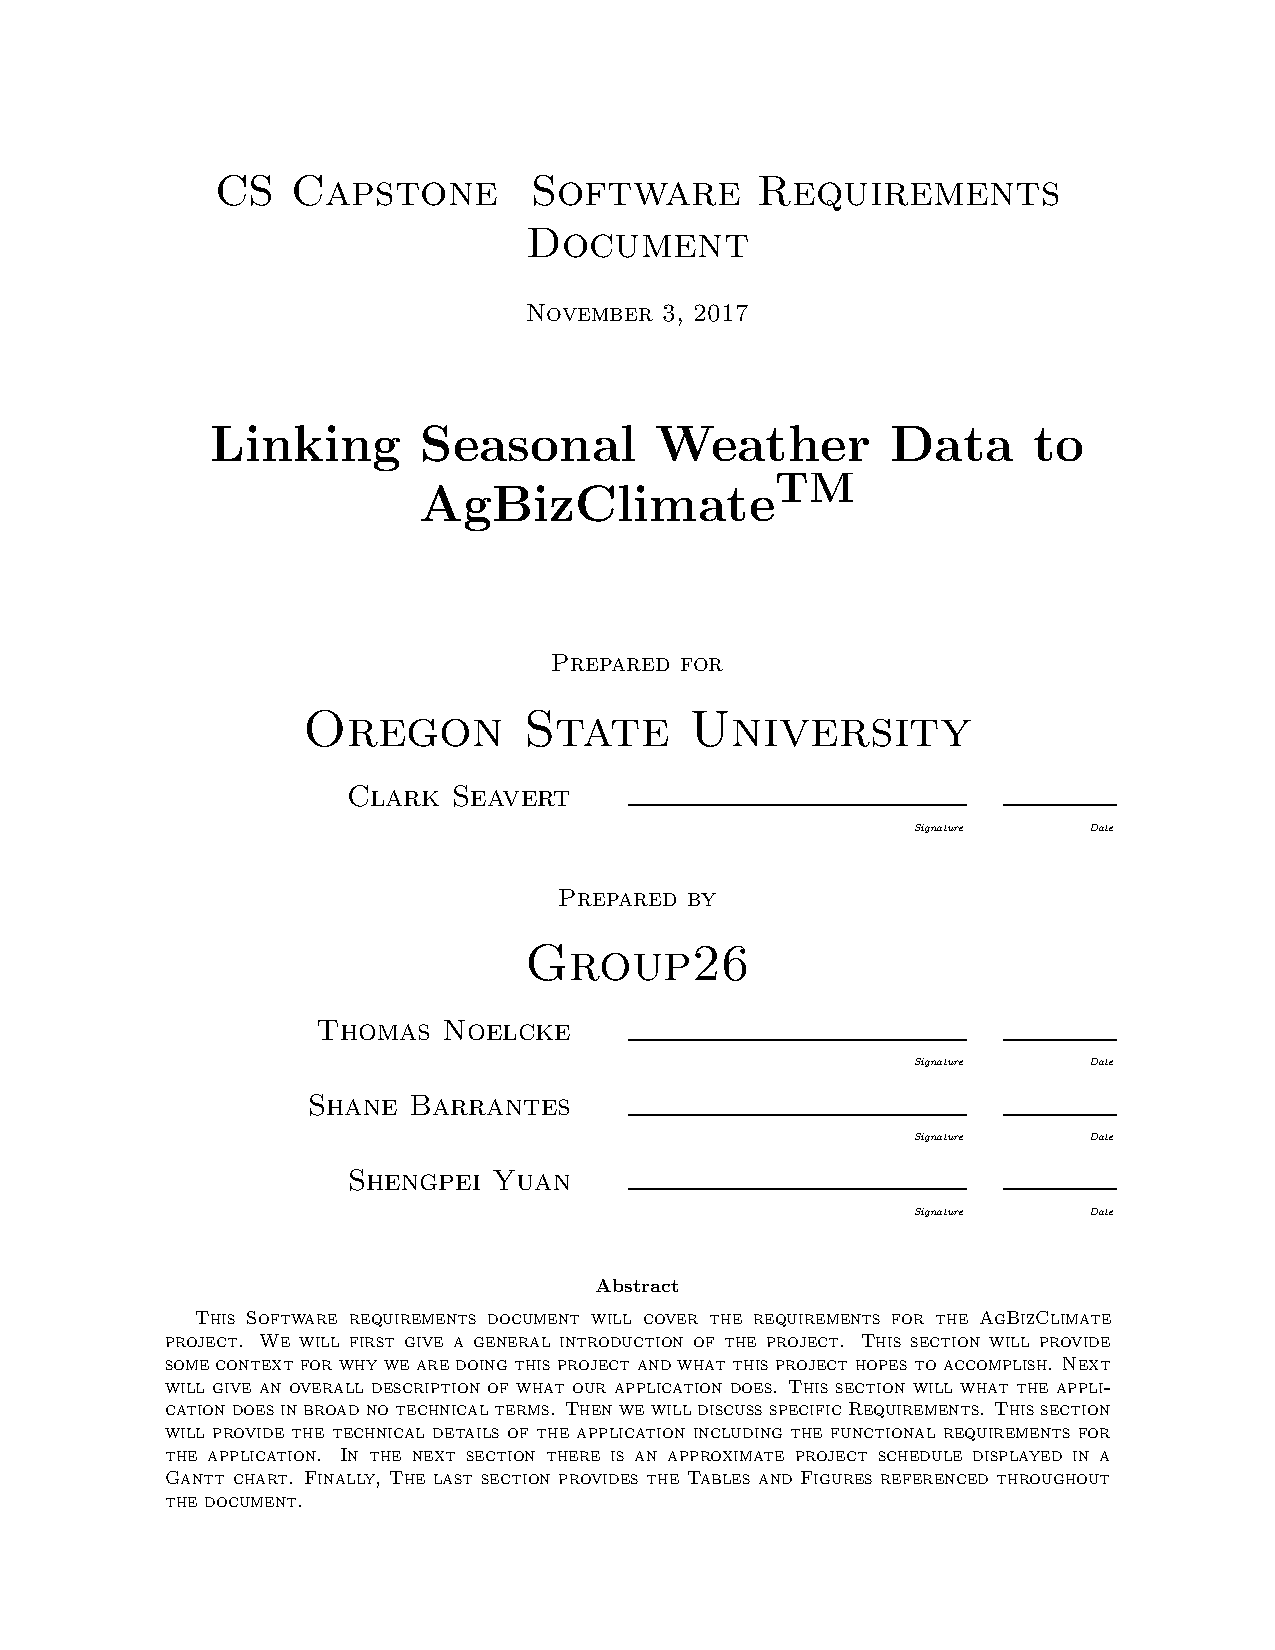
\includepdf[pages={1-16}]{./Original-Docs/Requirements-Document-Original/AgBizClimateSRS.pdf}
    
    \subsection{Changes}
\section{Design Document}
    \subsection{Original Document}
        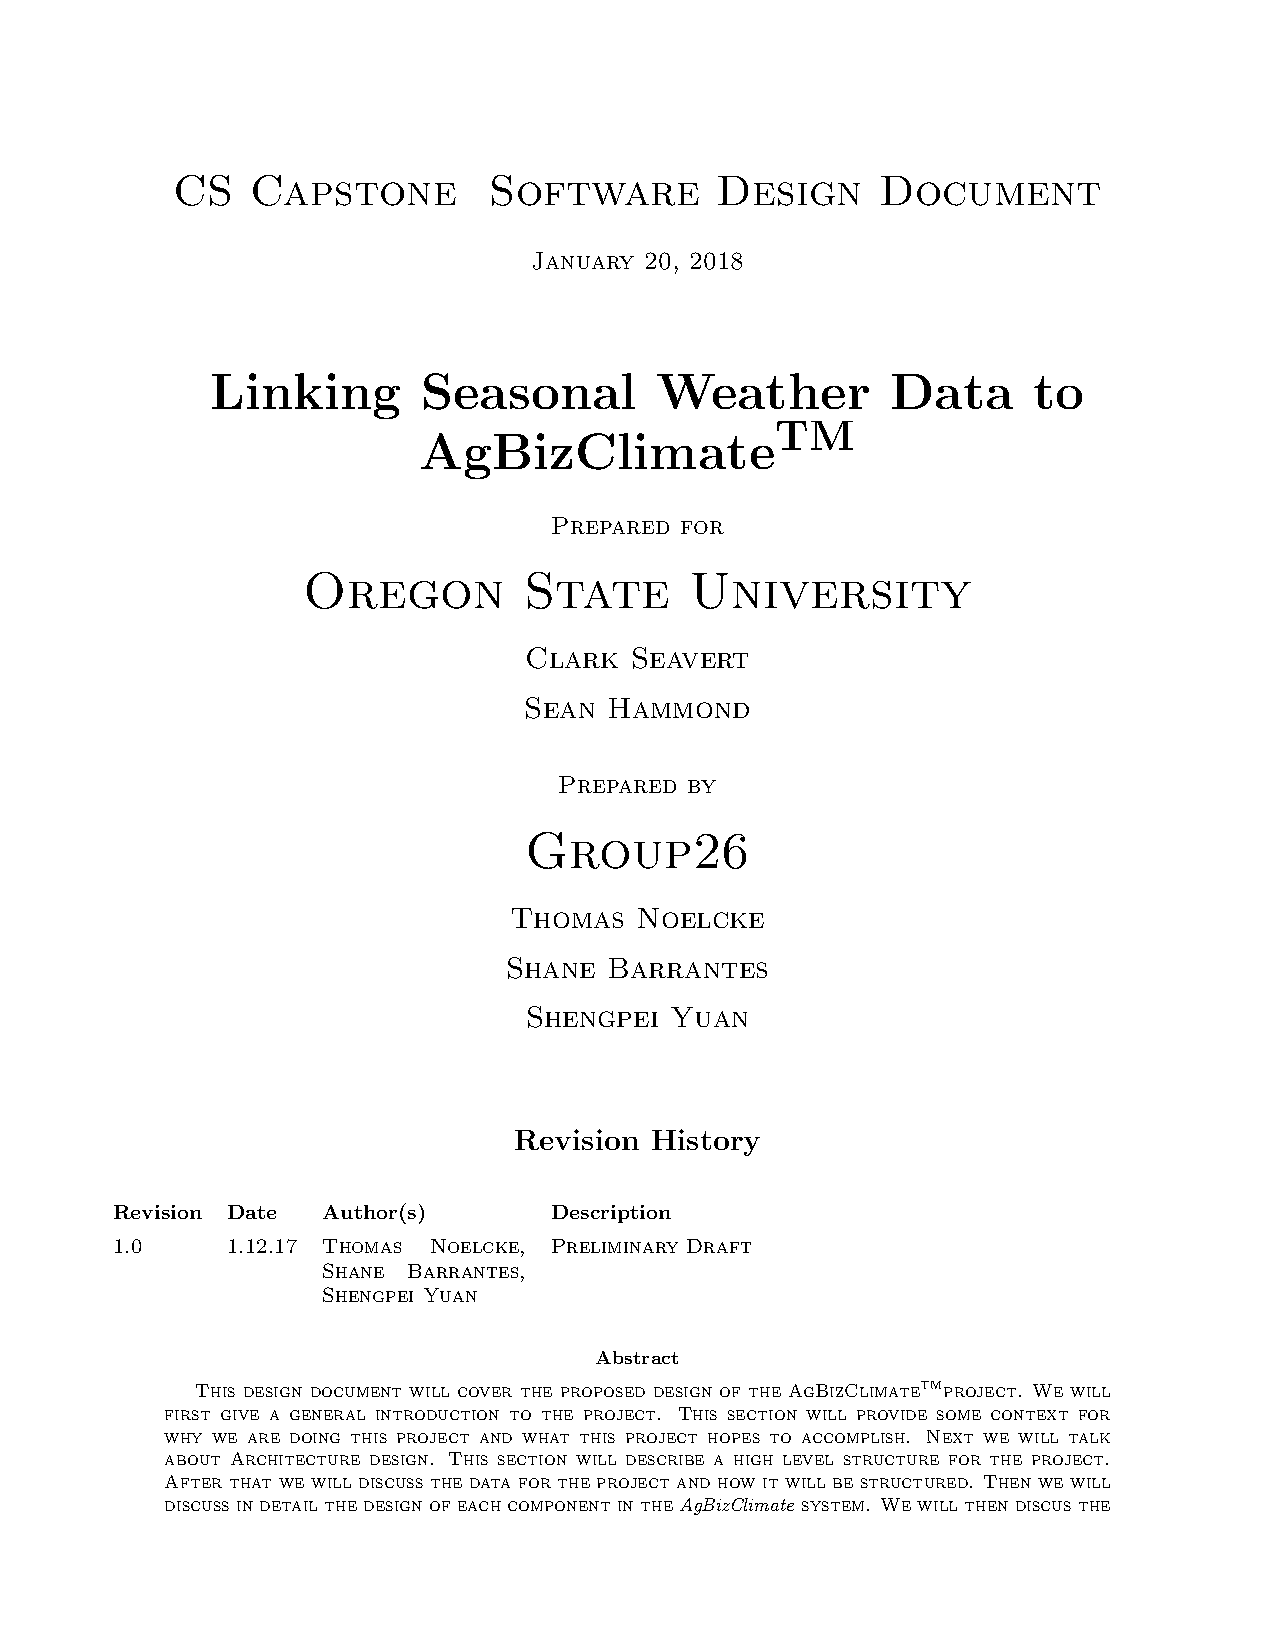
\includepdf[pages={1-33}]{./Original-Docs/DesignDoc/AgBizClimateDesignDoc.pdf}
    \subsection{Changes}
		
		
\section{Tech Review}
	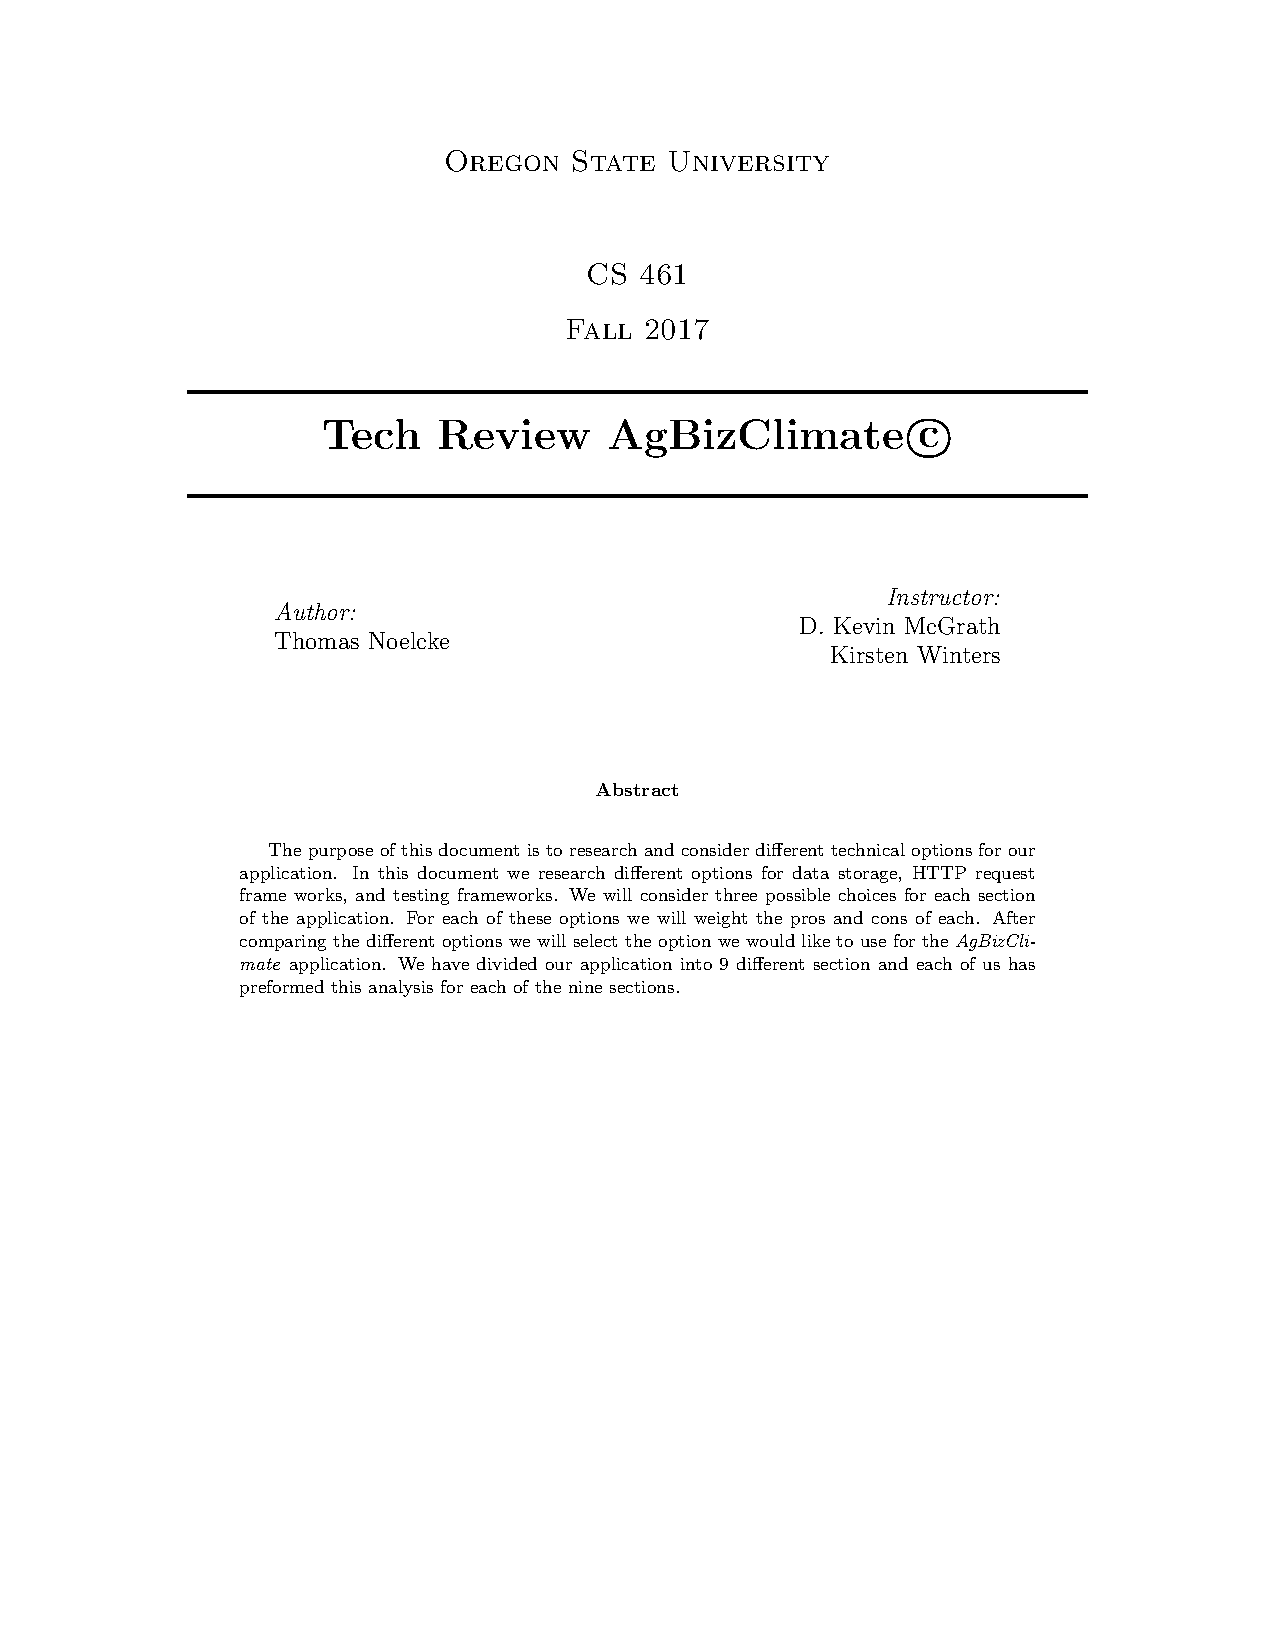
\includepdf[pages={1-23}]{./Original-Docs/Tech-Review/TechReviewCombined.pdf}

\section{Weekly Blog Posts}
    \subsection{Shane Barrantes}
    
    \subsection{Thomas Noelcke}
        In this section Will be every weekly update that I've made through out the term. It should be noted that I will denote the weeks by [term number].[week] where the week is the week number in the respective term and the term number represents the term. There will be 3 terms 1, 2 and 3 which will represent fall winter and spring respectively.\\ 
    
    \subsection{Shengpei Yuan}

\section{Final Poster}

%We will put set up and configuration steps here. We will also discuss how our project works. Hardware and software requirements. User guids, API Docs.
\section{Project Documentation}
    \subsection{Essential Documents}
    
    \subsection{Recommended Technical Resources}

\section{Conclusions and Reflections}
    \subsection{Shane Barrantes}
    
    \subsection{Thomas Noelcke}
    
    \subsection{Shengpei Yuan}

\section{Appendix}    

    \subsection{Appendix 1: Essential Code Listings}

    \subsection{Appendix 2: Catch all}
\end{document}
